\documentclass[aspectratio=169,10pt]{beamer}

\usetheme{Madrid}
\usecolortheme{seahorse}
\usefonttheme{professionalfonts}

\usepackage{amsmath,amssymb,amsthm}
\usepackage{mathtools}
\usepackage{listings}
\usepackage{xcolor}
\usepackage{booktabs}
\usepackage{graphicx}

\graphicspath{{figures/}}

%% Python style
\lstdefinestyle{python}{
  language=Python,
  basicstyle=\ttfamily\scriptsize,
  keywordstyle=\color{blue!80!black}\bfseries,
  stringstyle=\color{orange!80!black},
  commentstyle=\color{green!50!black}\itshape,
  numberstyle=\tiny\color{gray},
  numbers=left, stepnumber=1,
  frame=single, breaklines=true,
  showstringspaces=false, tabsize=4,
  backgroundcolor=\color{gray!7},
}

\title[MC Theory -- Ch.1]{Lectures on Monte Carlo Theory}
\subtitle{Chapter 1: Introduction}
\author{Based on Leskel\"{a} \& Vihola}
\date{}

\setbeamertemplate{navigation symbols}{}
\setbeamertemplate{footline}[frame number]

\begin{document}

% ------------------------------------------------------------------ title
\begin{frame}
  \titlepage
\end{frame}

% ------------------------------------------------------------------ TOC
\begin{frame}{Chapter Outline}
  \tableofcontents
\end{frame}

\section{1.1 About the Book}
\section{1.2 Simple Symmetric Random Walk}
\section{1.3 Travelling Salesman Problem}
\section{1.4 Computing Integrals with MC}
\section{1.5 Quasi-Monte Carlo Methods}
\section{1.6 MC vs Quasi-MC Comparison}
\section{1.7 Bibliographical Notes}

%% ==================================================================
\begin{frame}[allowframebreaks]{1.1 About the Book}

  \begin{block}{What is Monte Carlo (MC)?}
    \textbf{Monte Carlo methods} are computational algorithms that use
    \emph{random (pseudo-random) numbers} to solve mathematical and
    statistical problems --- integration, optimisation, and simulation
    of stochastic systems.
  \end{block}

  \textbf{Historical origin:} Developed at Los Alamos in the 1940s by
  von~Neumann, Ulam, and Metropolis for nuclear weapons simulation.
  Named after the Monte Carlo casino.

  \bigskip
  \textbf{Why randomness helps:}
  \begin{itemize}
    \item High-dimensional integrals: grid methods cost $n^d$ evaluations
      (exponential in dimension $d$).
    \item NP-hard combinatorial problems (TSP, knapsack).
    \item Complex stochastic systems with no closed-form solution.
    \item Bayesian posterior distributions.
  \end{itemize}

  \framebreak

  \textbf{Book contents:}
  \begin{enumerate}
    \item \textbf{Ch.1} Introduction: motivating examples
    \item \textbf{Ch.2} Theory of random number generators and statistical tests
    \item \textbf{Ch.3} Generating random variables
    \item \textbf{Ch.4} Output analysis: confidence intervals, estimators
    \item \textbf{Ch.5} Variance reduction (stratification, antithetic, IS, CE)
    \item \textbf{Ch.6} Markov Chain MC (Metropolis, Gibbs, CFTP)
    \item \textbf{Ch.7} Stochastic optimisation (simulated annealing, CE)
    \item \textbf{Ch.8} Simulation of queues and related processes
  \end{enumerate}

  \begin{alertblock}{Key distinction: MC vs Quasi-MC}
    \textbf{Monte Carlo} uses \emph{pseudo-random} sequences (deterministic
    but statistically random-looking). \textbf{Quasi-Monte Carlo (QMC)}
    uses carefully designed \emph{low-discrepancy} sequences that fill
    $[0,1]^d$ more evenly.
  \end{alertblock}

\end{frame}

\begin{frame}[fragile]{1.1 Pseudorandom Numbers in Python}

  \begin{block}{NumPy recommended API}
    Use \texttt{default\_rng} with an explicit seed for reproducibility.
    Successive calls produce statistically i.i.d.-looking numbers,
    but are entirely deterministic given the seed.
  \end{block}

\begin{lstlisting}[style=python]
import numpy as np
from numpy.random import PCG64, default_rng

rng  = np.random.default_rng(seed=1234)    # default PCG64 generator
rng2 = default_rng(PCG64(seed=1234))       # explicit generator

u1 = rng.random(5)   # 5 samples from Uniform[0,1)
u2 = rng.random(5)   # next 5 -- different values, same stream

steps = 1 - 2 * rng.integers(0, high=2, size=10)  # +1/-1 steps
print(steps)
\end{lstlisting}

  \textbf{The PCG64 generator} passes all standard statistical tests
  and has period $2^{128}$.  It is the default in NumPy $\ge 1.17$.

\end{frame}

%% ==================================================================
\begin{frame}[allowframebreaks]{1.2.1 Simple Symmetric Random Walk: Setup}

  \textbf{Motivating game (Feller):} Two players A and B bet on coin tosses.
  A wins $+1$ on heads, $-1$ on tails. Starting fortune $S_0 = 0$.

  \begin{block}{Definition --- Simple Symmetric Random Walk (SSRW)}
    Let $X_1, X_2, \ldots$ be i.i.d.\ with
    $\mathbb{P}(X_j = +1) = \mathbb{P}(X_j = -1) = \tfrac{1}{2}$.
    \[
      S_0 = 0, \qquad S_n = \sum_{j=1}^{n} X_j, \quad n \ge 1.
    \]
  \end{block}

  \textbf{Questions about $(S_n)_{n=0,\ldots,2N}$:}
  \begin{description}
    \item[Q1] $L_{2N} = \max\{i : S_i = 0\}$ --- last tie. Distribution?
    \item[Q2] $P(\alpha,\beta)$ --- fraction of time A is winning?
    \item[Q3] How do the oscillations of $S_n$ grow?
    \item[Q4] Probability one player is \emph{always} winning?
  \end{description}

  \framebreak

  \begin{center}
    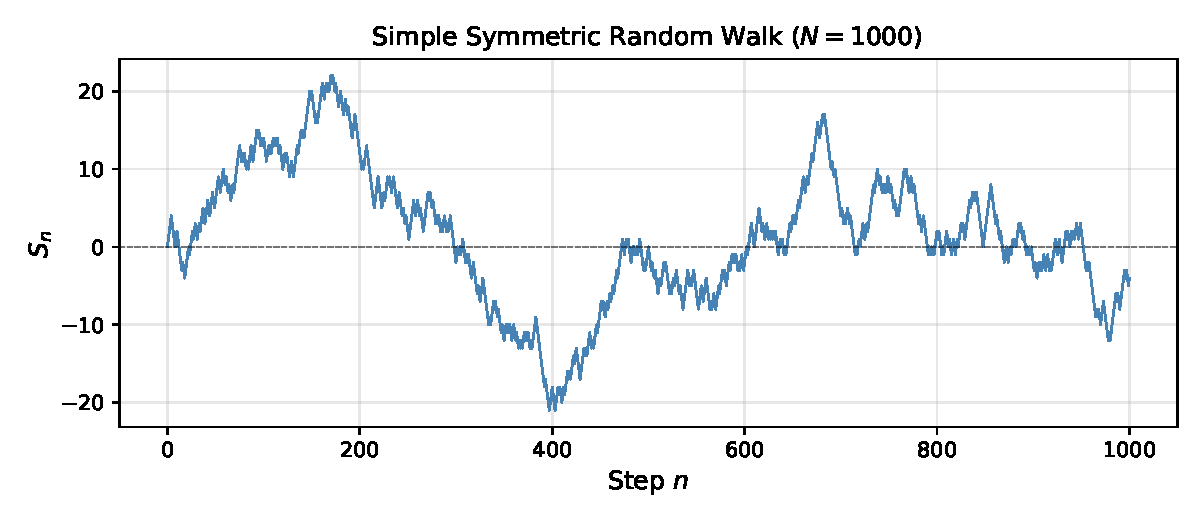
\includegraphics[width=0.88\textwidth]{fig_ssrw_single}
  \end{center}
  \textit{A single realisation of the SSRW for $N=1000$ steps.
  The walk frequently crosses zero but also has long excursions on one side.}

\end{frame}

%% ------------------------------------------------------------------
\begin{frame}[allowframebreaks]{1.2.1 Key Quantities of the SSRW}

  \begin{block}{Last time at zero}
    \[
      L_{2n} = \sup\{m \le 2n : S_m = 0\}
    \]
  \end{block}

  \begin{block}{Steps spent on or above zero}
    \[
      L^+_{2n} = \#\{j = 1, \ldots, 2n : S_{j-1} \ge 0 \;\text{or}\; S_j \ge 0\}
    \]
    A segment from $(j-1, S_{j-1})$ to $(j, S_j)$ is \emph{above} the axis
    if either endpoint is non-negative.
  \end{block}

  \begin{exampleblock}{Intuition check}
    By symmetry one might expect $L^+_{2n}/(2n) \approx 1/2$. The
    \textbf{Arcsine Law} shows this is wrong: most mass is near 0 and 1!
  \end{exampleblock}

  \framebreak

  \begin{block}{Law of the Iterated Logarithm (LIL)}
    \[
      \mathbb{P}\!\left(\liminf_{n\to\infty}
        \frac{S_n}{\sqrt{2n\log\log n}} = -1\right)
      = \mathbb{P}\!\left(\limsup_{n\to\infty}
        \frac{S_n}{\sqrt{2n\log\log n}} = +1\right) = 1.
    \]
  \end{block}

  \begin{columns}[T]
    \begin{column}{0.46\textwidth}
      \textbf{Three scales for $S_n$:}
      \begin{itemize}
        \item $S_n / n \to 0$: \textit{too strong}
        \item $S_n / \sqrt{n}$: \textit{too weak} (oscillates $\to\infty$)
        \item $S_n / \sqrt{2n\log\log n}$: \textbf{exact} \\
          $\limsup = +1$, $\liminf = -1$ a.s.
      \end{itemize}
    \end{column}
    \begin{column}{0.50\textwidth}
      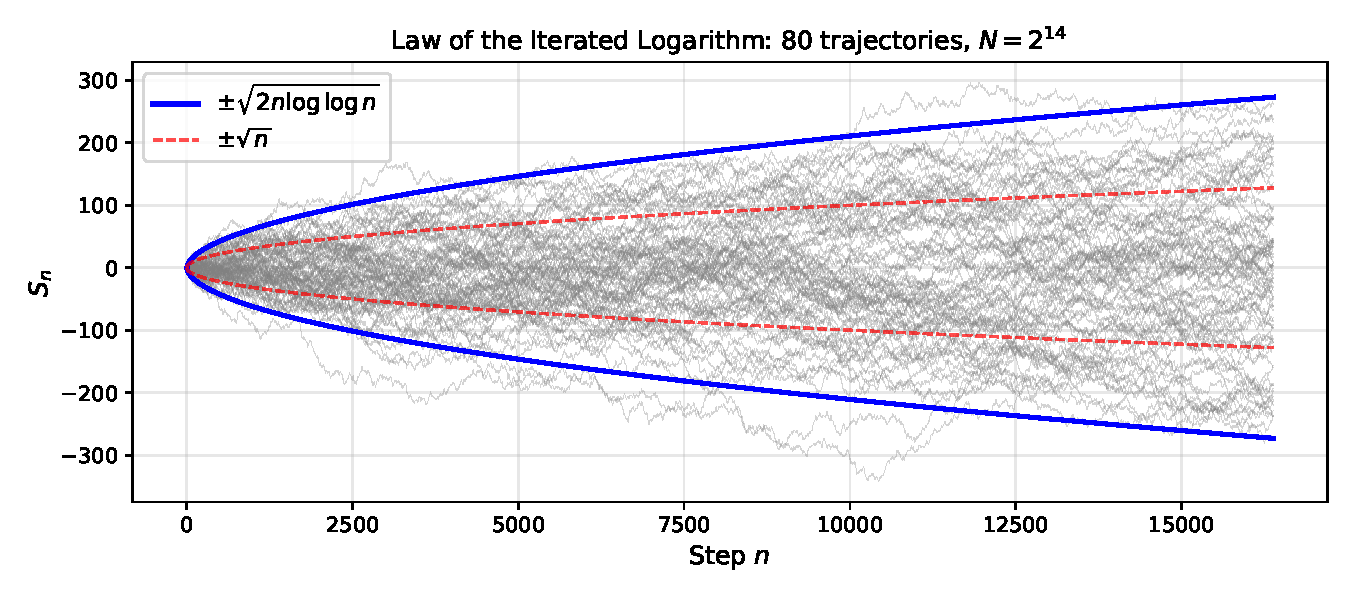
\includegraphics[width=\textwidth]{fig_lil_envelope}
    \end{column}
  \end{columns}

  \vspace{0.3em}
  \textit{80 independent trajectories ($N=2^{14}$). Blue: LIL envelope
  $\pm\sqrt{2n\log\log n}$. Red dashed: $\pm\sqrt{n}$ for comparison.
  Paths stay inside the LIL band and touch it infinitely often.}

\end{frame}

%% ------------------------------------------------------------------
\begin{frame}[fragile]{1.2.1 Python: Simulating the SSRW}

\begin{lstlisting}[style=python]
import numpy as np
import matplotlib.pyplot as plt
from numpy.random import default_rng

rng, N = default_rng(seed=31415), 1000

steps = 1 - 2 * rng.integers(0, high=2, size=N)  # +1 or -1
S     = np.concatenate([[0], steps.cumsum()])

# LIL envelope
n_arr    = np.arange(1, N + 1)
envelope = np.sqrt(2 * n_arr * np.log(np.log(n_arr + 2)))

fig, ax = plt.subplots(figsize=(9, 3.5))
ax.plot(S, lw=0.9, color='steelblue', label='$S_n$')
ax.plot(n_arr,  envelope, 'b-', lw=1.8, label=r'$\pm\sqrt{2n\log\log n}$')
ax.plot(n_arr, -envelope, 'b-', lw=1.8)
ax.axhline(0, color='k', lw=0.5, ls='--')
ax.set_xlabel('Step $n$'); ax.set_ylabel('$S_n$')
ax.legend(); ax.grid(True, alpha=0.3); plt.tight_layout(); plt.show()
\end{lstlisting}

\end{frame}

%% ------------------------------------------------------------------
\begin{frame}[allowframebreaks]{1.2.1 The Arcsine Law}

  \begin{block}{Arcsine Law}
    For $0 \le \alpha < \beta \le 1$:
    \[
      \mathbb{P}\!\left(\alpha \le \frac{L^+_{2n}}{2n} \le \beta\right)
      \;\xrightarrow{n\to\infty}\;
      \int_\alpha^\beta \frac{dx}{\pi\sqrt{x(1-x)}}.
      \tag{1.2.1}
    \]
    A similar result holds for $L_{2n}$.
  \end{block}

  \textbf{Why ``arcsine''?}
  \[
    \int_0^\beta \frac{dx}{\pi\sqrt{x(1-x)}}
    = \frac{2}{\pi}\arcsin\!\bigl(\sqrt{\beta}\bigr).
  \]
  The density $p(x) = (\pi\sqrt{x(1-x)})^{-1}$ is \textbf{U-shaped}:
  it is $\to\infty$ at $x=0$ and $x=1$, with minimum at $x=1/2$.
  The walk spends most time entirely above \emph{or} entirely below zero.

  \framebreak

  \begin{center}
    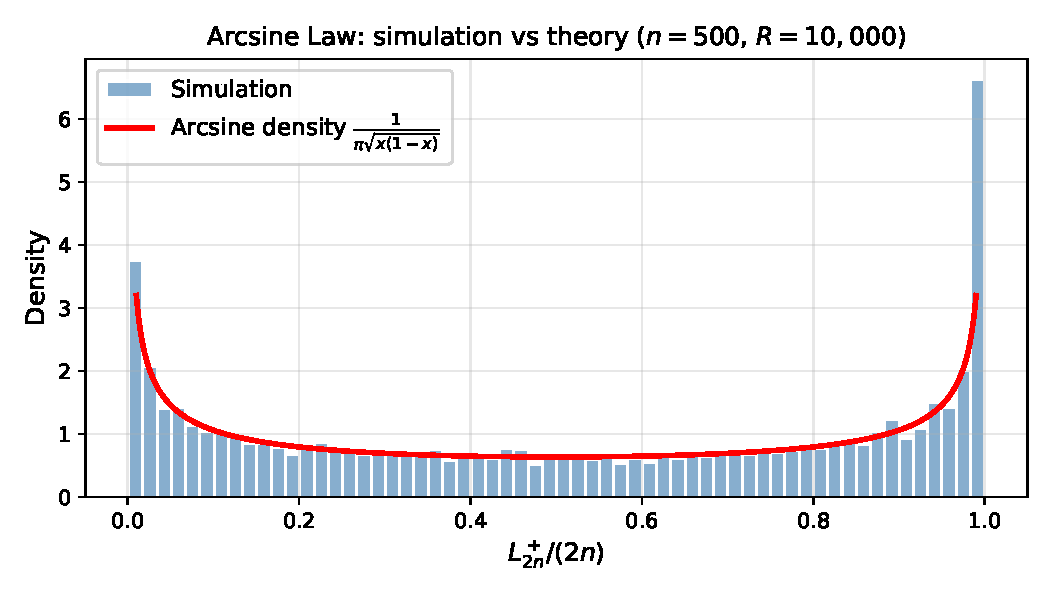
\includegraphics[width=0.72\textwidth]{fig_arcsine_law}
  \end{center}
  \textit{Histogram of $L^+_{2n}/(2n)$ from $R=10{,}000$ independent
  replications with $n=500$.  The empirical distribution closely matches
  the theoretical arcsine density (red curve). The U-shape confirms:
  nearly all time above or nearly all time below zero is most likely.}

\end{frame}

\begin{frame}[fragile]{1.2.1 Python: Verifying the Arcsine Law}

\begin{lstlisting}[style=python]
import numpy as np, matplotlib.pyplot as plt

def fraction_positive(n, R=10_000, seed=0):
    rng   = np.random.default_rng(seed)
    steps = 1 - 2 * rng.integers(0, 2, (R, 2*n))
    S     = np.hstack([np.zeros((R,1)), steps.cumsum(axis=1)])
    # L+: step j counted if S_{j-1}>=0 OR S_j>=0
    above = (S[:, :-1] >= 0) | (S[:, 1:] >= 0)
    return above.sum(axis=1) / (2*n)

fracs = fraction_positive(n=500)
x     = np.linspace(0.01, 0.99, 400)
pdf   = 1.0 / (np.pi * np.sqrt(x * (1 - x)))

plt.figure(figsize=(7,4))
plt.hist(fracs, bins=60, density=True, alpha=0.65, label='Simulation')
plt.plot(x, pdf, 'r-', lw=2.2,
         label=r'Arcsine density $\frac{1}{\pi\sqrt{x(1-x)}}$')
plt.xlabel(r'$L^+_{2n}/(2n)$'); plt.ylabel('Density')
plt.legend(); plt.tight_layout(); plt.show()
\end{lstlisting}

\end{frame}

%% ==================================================================
\begin{frame}[allowframebreaks]{1.3 Travelling Salesman Problem}

  \begin{block}{Problem}
    Given $n$ cities with pairwise distances $d(c_i, c_j)$, find the
    shortest closed tour:
    \[
      \pi^* = \arg\min_{\pi \in S_n}
        \sum_{i=1}^{n} d\!\bigl(c_{\pi(i)}, c_{\pi(i+1)}\bigr),
      \quad c_{\pi(n+1)} \coloneqq c_{\pi(1)}.
    \]
  \end{block}

  \textbf{Why is it hard?}
  \begin{itemize}
    \item \textbf{NP-complete}: no polynomial algorithm known.
    \item Search space: $n!$ permutations. For $n=20$: $\approx 2.4\times10^{18}$.
    \item Exact solvers only feasible for $n \lesssim 50$.
  \end{itemize}

  \textbf{MC heuristics:}
  \begin{itemize}
    \item Random restart: sample many tours, keep the shortest.
    \item \textbf{Simulated Annealing} (Ch.~7): accept worse solutions
      probabilistically to escape local optima.
    \item \textbf{Cross-Entropy method} (Chs.~5, 7): fit a distribution over
      tours, iteratively resample and improve.
  \end{itemize}

  \framebreak

  \begin{center}
    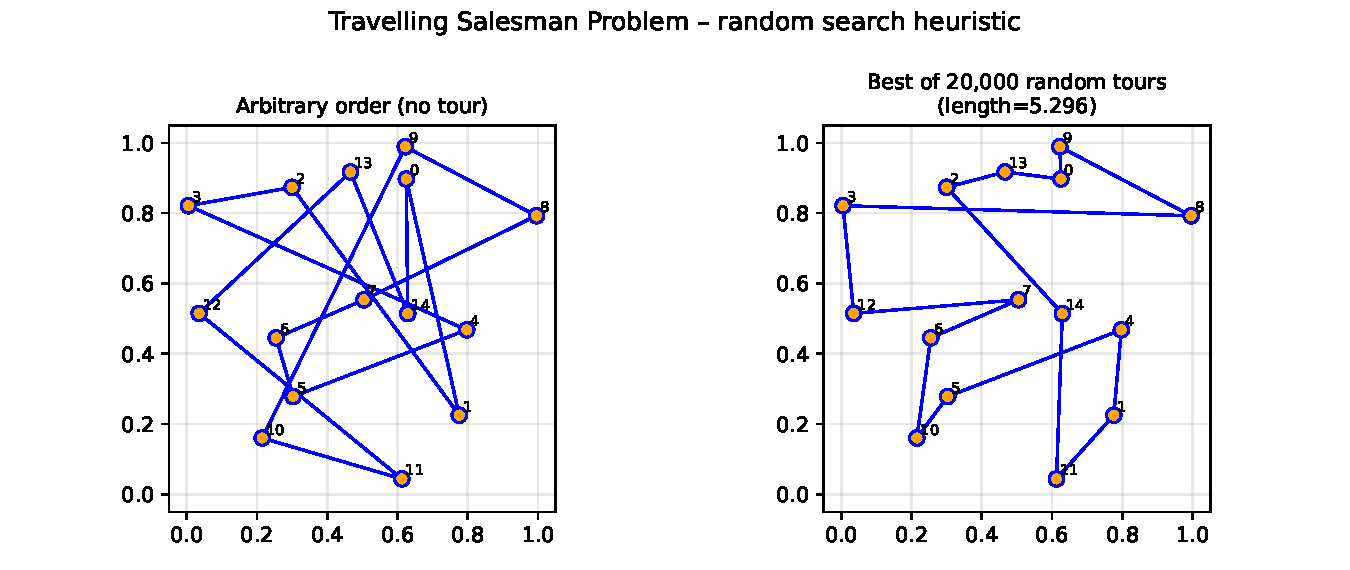
\includegraphics[width=0.85\textwidth]{fig_tsp}
  \end{center}
  \textit{Left: arbitrary city order (no tour optimisation). Right: best
  tour found by random search over 20{,}000 permutations for 15 random cities.
  The key idea: randomness helps explore the space; SA/CE methods (Ch.~7)
  do much better by using intelligent proposals.}

\end{frame}

\begin{frame}[fragile]{1.3 Python: Random Tour Search}

\begin{lstlisting}[style=python]
import numpy as np

def tour_length(cities, perm):
    shifted = np.roll(perm, -1)
    return np.linalg.norm(cities[perm] - cities[shifted], axis=1).sum()

def random_tour_search(cities, R=20_000, seed=42):
    rng = np.random.default_rng(seed)
    n   = len(cities)
    best_len, best_tour = np.inf, None
    for _ in range(R):
        perm = rng.permutation(n)
        L    = tour_length(cities, perm)
        if L < best_len:
            best_len, best_tour = L, perm.copy()
    return best_tour, best_len

rng    = np.random.default_rng(7)
cities = rng.random((15, 2))   # 15 random 2-D cities
tour, length = random_tour_search(cities)
print(f"Best tour (random search, R=20000): {length:.4f}")
# This is a weak baseline; simulated annealing (Ch.7) does much better.
\end{lstlisting}

\end{frame}

%% ==================================================================
\begin{frame}[allowframebreaks]{1.4 Computing Integrals with Monte Carlo}

  \textbf{Goal:} Estimate $I = \int_{[0,1]^d} f(\mathbf{u})\,d\mathbf{u}
  = \mathbb{E}[f(\mathbf{U})]$, $\mathbf{U}\sim\mathrm{Uniform}[0,1]^d$.

  \begin{block}{Monte Carlo Estimator}
    Sample $\mathbf{U}_1,\ldots,\mathbf{U}_R \overset{\text{i.i.d.}}{\sim}
    \mathrm{Uniform}[0,1]^d$, set $Z_i = f(\mathbf{U}_i)$:
    \[
      \hat{I}_R = \frac{1}{R}\sum_{i=1}^{R} Z_i
      \;\xrightarrow{R\to\infty}\; I \quad\text{(SLLN)}.
    \]
  \end{block}

  \begin{block}{Variance and CLT}
    \[
      \mathrm{Var}(\hat{I}_R) = \frac{\sigma^2}{R},
      \qquad \sigma^2 = \mathrm{Var}(f(\mathbf{U})).
    \]
    \[
      \sqrt{R}(\hat{I}_R - I) \xrightarrow{d} \mathcal{N}(0,\sigma^2).
      \quad \Rightarrow \quad
      \text{RMSE} = \frac{\sigma}{\sqrt{R}} = \mathcal{O}(R^{-1/2}).
    \]
  \end{block}

  \framebreak

  \textbf{Why this is remarkable --- dimension-free convergence:}

  \begin{center}
  \begin{tabular}{lll}
    \toprule
    Method & Error & Evaluations for $\varepsilon=10^{-2}$, $d=10$ \\
    \midrule
    Grid ($n^d$ points) & $\mathcal{O}(n^{-2/d})$ & $100^{10} = 10^{20}$ \\
    Monte Carlo         & $\mathcal{O}(R^{-1/2})$  & $\sim 10^4$ \\
    \bottomrule
  \end{tabular}
  \end{center}

  For $d \ge 5$, Monte Carlo is almost always preferred over grid quadrature.

  \vspace{0.5em}
  \textbf{Discrepancy:} The error in the estimator is also bounded by the
  \emph{discrepancy} of the sample:
  \[
    D(\mathbf{x}_1,\ldots,\mathbf{x}_n)
    = \sup_{B \subseteq [0,1]^d}
      \left|\frac{\#\{i:\mathbf{x}_i\in B\}}{n} - \lambda(B)\right|.
  \]
  For i.i.d.\ uniform: $D = \mathcal{O}(n^{-1/2})$. This motivates QMC.

\end{frame}

\begin{frame}[fragile]{1.4 Python: Estimating $\pi$ with MC}

\begin{lstlisting}[style=python]
import numpy as np

def estimate_pi(R, seed=0):
    rng    = np.random.default_rng(seed)
    U      = rng.random((R, 2))
    inside = (U**2).sum(axis=1) <= 1.0   # inside unit quarter-circle
    return 4.0 * inside.mean()

# Area of quarter unit disk = pi/4; multiply by 4 to get pi
for R in [100, 1_000, 10_000, 100_000, 1_000_000]:
    pi_hat = estimate_pi(R)
    print(f"R={R:>9,}  pi_hat={pi_hat:.5f}  "
          f"|error|={abs(pi_hat - np.pi):.5f}")
# Each 100x increase in R => ~10x reduction in error (sqrt rule)
\end{lstlisting}

  \begin{exampleblock}{Convergence rate}
    RMSE $= \sigma/\sqrt{R} = \mathcal{O}(R^{-1/2})$.
    Multiply $R$ by 100 $\Rightarrow$ error shrinks by factor $\approx 10$.
  \end{exampleblock}

\end{frame}

%% ==================================================================
\begin{frame}[allowframebreaks]{1.5 Quasi-Monte Carlo (QMC) Methods}

  \begin{block}{Idea}
    Replace i.i.d.\ random points with a \textbf{deterministic, well-spread}
    sequence that covers $[0,1]^d$ more uniformly.
  \end{block}

  \begin{block}{Low-discrepancy bound}
    Several constructive sequences achieve:
    \[
      D(\mathbf{x}_1,\ldots,\mathbf{x}_n) \le
      C_d\,\frac{(\log n)^d}{n} + \mathcal{O}\!\left(\frac{(\log n)^{d-1}}{n}\right).
    \]
    Compare to MC: $D = \mathcal{O}(n^{-1/2})$.
  \end{block}

  \begin{block}{Koksma--Hlawka inequality}
    If $V(f)$ is the Hardy--Krause variation of $f$:
    \[
      \left|\hat{I}_n^{\mathrm{QMC}} - I\right|
      \le V(f) \cdot D(\mathbf{x}_1,\ldots,\mathbf{x}_n)
      = \mathcal{O}\!\left(\frac{(\log n)^d}{n}\right).
    \]
  \end{block}

  \framebreak

  \textbf{Popular low-discrepancy sequences (all in \texttt{scipy.stats.qmc}):}

  \begin{description}
    \item[Halton] Van der Corput sequences with different prime bases per
      dimension. Simple; mild correlations for large primes.
    \item[Sobol'] Constructed via bit operations. Excellent for $d\ge2$;
      works best when $n = 2^k$.
    \item[Faure] Permuted base-$p$ sequences. Proven bounds.
    \item[Latin Hypercube] Each row/column of the grid has exactly one
      sample. Good uniformity but not strictly low-discrepancy.
  \end{description}

  \begin{center}
    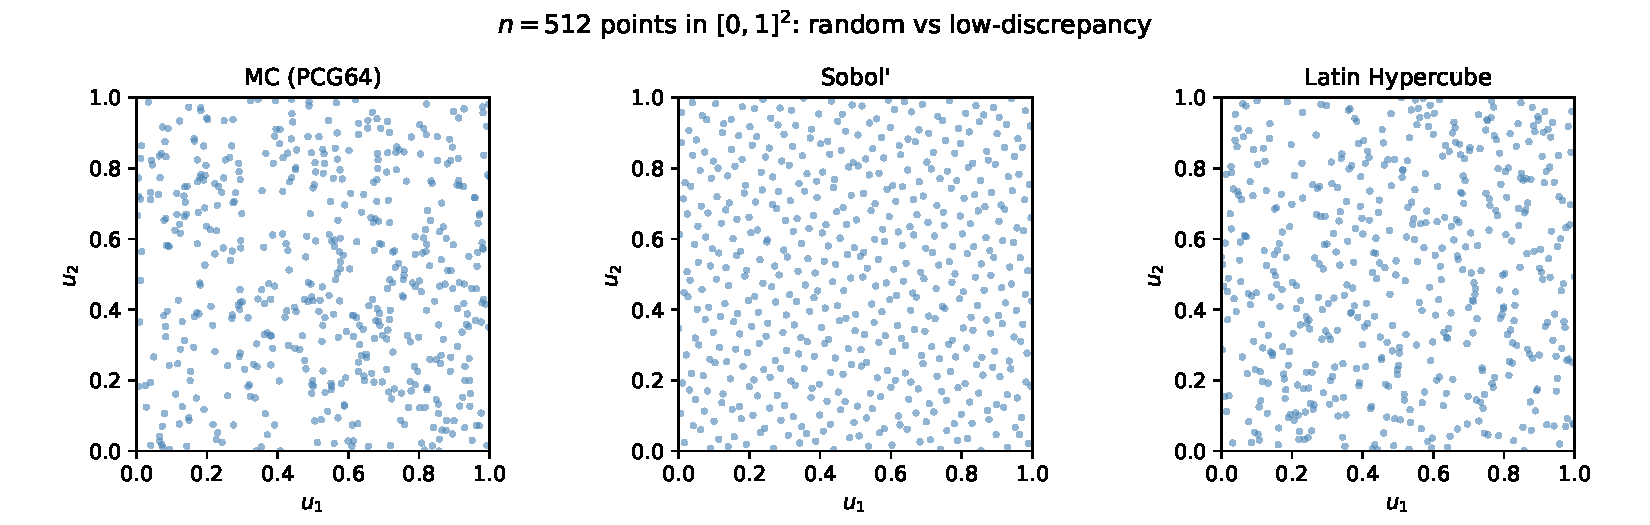
\includegraphics[width=0.85\textwidth]{fig_mc_vs_qmc_scatter}
  \end{center}
  \textit{$n=512$ points in $[0,1]^2$. Left: MC (PCG64) --- visible clusters
  and gaps. Centre: Sobol' --- noticeably more uniform. Right: Latin
  Hypercube --- each column/row subdivided evenly.}

  \framebreak

  \begin{block}{Golden-ratio (Steinhaus) sequence -- 1D}
    \[
      x_n = \{n\alpha\}, \qquad
      \alpha = \frac{\sqrt{5}-1}{2} \approx 0.6180
      \quad\text{(golden ratio)},
    \]
    $\alpha$ is the solution of $z^2+z-1=0$ with continued-fraction expansion
    $\alpha = \cfrac{1}{1+\cfrac{1}{1+\cdots}}$.
    This makes $\alpha$ the ``most irrational'' number, giving maximal spread.
  \end{block}

  \begin{block}{Kronecker sequences}
    $x_n = \{n\beta\}$ has low discrepancy when the partial quotients
    of $\beta$'s continued fraction are bounded.
    Multidimensional Kronecker sequences
    $(\{n\beta_1\},\ldots,\{n\beta_d\})$ are an open problem but
    numerical evidence is positive.
  \end{block}

  \begin{alertblock}{Remark on multidimensional QMC}
    Grouping consecutive 1-D low-discrepancy numbers into $d$-dimensional
    vectors \textbf{does not} preserve the low-discrepancy property.
    Each dimension must be constructed simultaneously (as \texttt{scipy.stats.qmc} does).
  \end{alertblock}

\end{frame}

\begin{frame}[fragile]{1.5 Python: QMC with \texttt{scipy.stats.qmc}}

\begin{lstlisting}[style=python]
import numpy as np
from scipy.stats.qmc import Sobol, Halton, LatinHypercube

def pi_from(U):
    return 4.0 * ((U**2).sum(1) <= 1).mean()

Rs = [2**k for k in range(4, 15)]   # 16 ... 16384
mc_err, sob_err, hal_err = [], [], []
for R in Rs:
    rng = np.random.default_rng(0)
    mc_err.append( abs(pi_from(rng.random((R,2))) - np.pi))
    sob_err.append(abs(pi_from(Sobol(2, scramble=True,  seed=0).random(R)) - np.pi))
    hal_err.append(abs(pi_from(Halton(2, scramble=True, seed=0).random(R)) - np.pi))

import matplotlib.pyplot as plt
plt.loglog(Rs, mc_err,  'b-o', label='MC (PCG64)')
plt.loglog(Rs, sob_err, 'r-s', label="Sobol'")
plt.loglog(Rs, hal_err, 'g-^', label='Halton')
ref = [mc_err[0] * (Rs[0]/r)**0.5 for r in Rs]
plt.loglog(Rs, ref, 'k--', label=r'$O(R^{-1/2})$')
plt.xlabel('R'); plt.ylabel('|error|'); plt.legend(); plt.grid(True)
plt.title(r'MC vs QMC convergence to $\pi$')
plt.tight_layout(); plt.show()
\end{lstlisting}

\end{frame}

%% ==================================================================
\begin{frame}[allowframebreaks]{1.6 MC vs Quasi-MC: Convergence Comparison}

  \begin{columns}[T]
    \begin{column}{0.52\textwidth}
      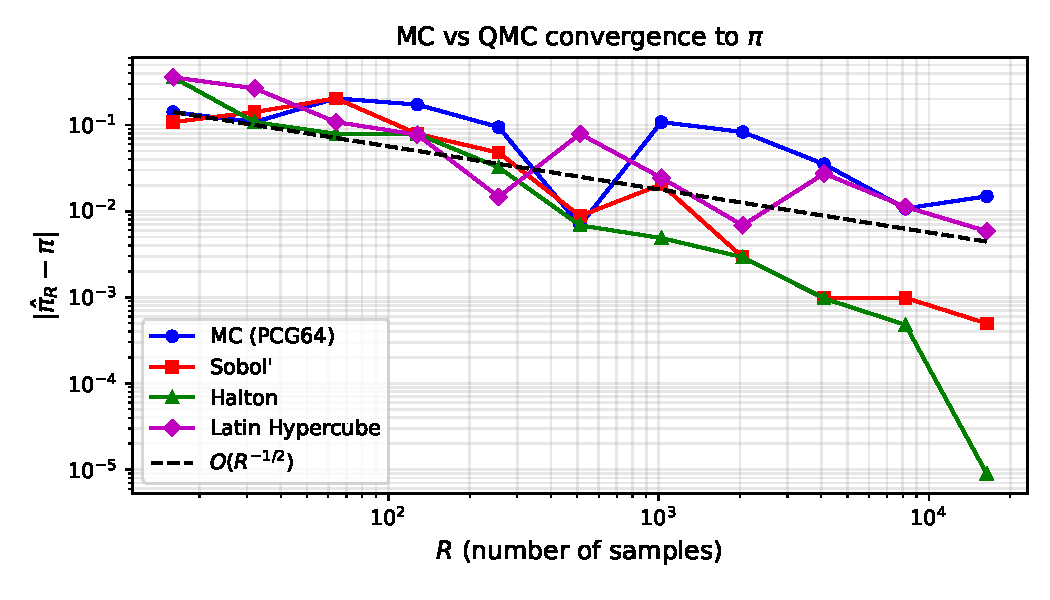
\includegraphics[width=\textwidth]{fig_convergence_pi}
    \end{column}
    \begin{column}{0.45\textwidth}
      \textbf{Estimating $\pi$ via MC/QMC:}
      \begin{itemize}
        \item Sobol' and Halton errors are much smaller for small $R$.
        \item All methods converge; QMC is faster for smooth $f$.
        \item The $O(R^{-1/2})$ reference slope matches MC well.
        \item QMC slope is steeper (faster), around $O(R^{-1})$ for this smooth integrand.
      \end{itemize}
    \end{column}
  \end{columns}

  \framebreak

  \begin{block}{Example 1.4.2 -- Winning Probability in a 2-D Game}
    Grid $\{0,\ldots,N_1\}\times\{0,\ldots,N_2\}$. From $(i_1,i_2)$:
    \begin{itemize}
      \item Any coordinate hits 0 $\Rightarrow$ \textbf{LOSE}
      \item Both coordinates reach $N_j$ $\Rightarrow$ \textbf{WIN}
    \end{itemize}
  \end{block}

  \begin{center}
    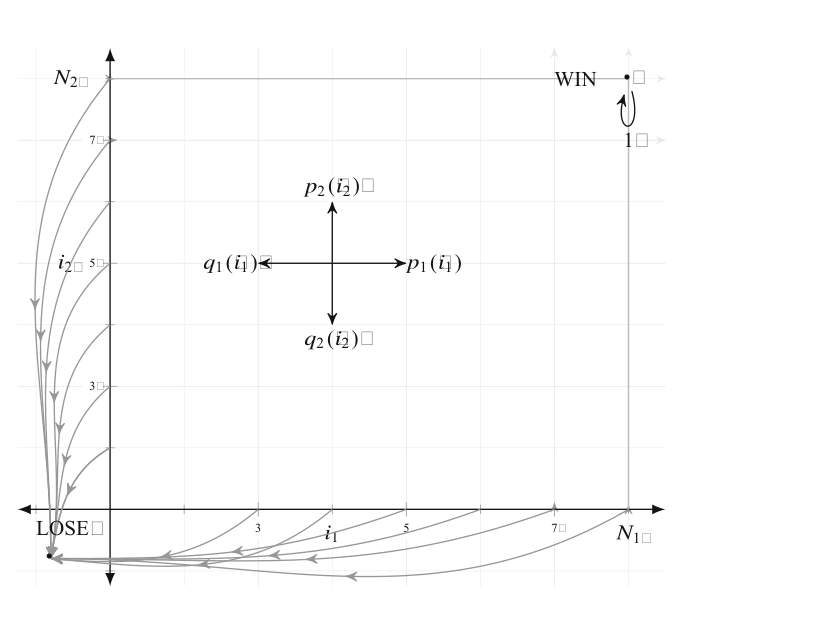
\includegraphics[width=0.52\textwidth]{fig_2d_game_grid_crop}
  \end{center}
  \textit{State-space of the 2-D game. Arrows show the four possible moves
  from state $(i_1,i_2)$ with probabilities $p_1,q_1,p_2,q_2$.
  LOSE corner: $(0,0)$; WIN corner: $(N_1,N_2)$.}

  \framebreak

  \begin{block}{Exact winning probability (Formula 1.4.1)}
    \[
      \rho(i_1, i_2) =
      \frac{\displaystyle
        \prod_{j=1}^{2}\!\left(\sum_{n_j=1}^{i_j}
          \prod_{r=1}^{n_j-1}\frac{q_j(r)}{p_j(r)}\right)}
      {\displaystyle
        \prod_{j=1}^{2}\!\left(\sum_{n_j=1}^{N_j}
          \prod_{r=1}^{n_j-1}\frac{q_j(r)}{p_j(r)}\right)},
    \]
    where empty products equal~1.
  \end{block}

  \textbf{Formula explanation:}
  \begin{itemize}
    \item The numerator sums over positions $1,\ldots,i_j$ for each player: it
      counts the ``probability weight'' of reaching the current position.
    \item The denominator normalises over all positions $1,\ldots,N_j$:
      the total weight to reach WIN.
    \item The product over $j=1,2$ reflects independence of the two coordinates.
  \end{itemize}

  \textbf{Symmetric case:} $N_1=N_2=4$, $p_j = q_j = 1/4$ gives
  $\rho(2,3) = 3/8 = 0.375$.

  \framebreak

  \textbf{Simulation algorithm --- one game from $(i_1, i_2)$:}

  Draw two uniforms $U_1, U_2 \in [0,1)$ per step:
  \begin{enumerate}
    \item \textbf{Which coordinate?} Use $U_1$:
      \begin{itemize}
        \item Coord.~1 if $U_1 \in [0,\; p_1+q_1)$
        \item Coord.~2 if $U_1 \in [p_1+q_1,\; p_1+q_1+p_2+q_2)$
        \item No move otherwise
      \end{itemize}
    \item \textbf{Which direction?} Use $U_2$:
      \begin{itemize}
        \item Coord.~1 up if $U_2 < p_1/(p_1+q_1)$, else down
        \item Coord.~2 up if $U_2 < p_2/(p_2+q_2)$, else down
      \end{itemize}
    \item Stop when any coord $= 0$ (LOSE) or all coords $= N_j$ (WIN).
  \end{enumerate}

  \textbf{Estimator:}
  $\;\hat{Y}_R^{A_i} = \frac{1}{R}\sum_{j=1}^{R} Y_j^{A_i}$,
  $\;Y_j^{A_i}\in\{0,1\}$,
  with $A_1=$PCG64, $A_2=$LatHyp, $A_3=$Sobol', $A_4=$Halton.

  \framebreak

  \begin{columns}[T]
    \begin{column}{0.48\textwidth}
      \begin{block}{Results: estimates of $\rho(2,3)=0.375$}
        \centering\small
        \begin{tabular}{rcccc}
          \toprule
          $R$ & PCG64 & LatHyp & Sobol & Halton \\
          \midrule
          1\,000 & 0.3760 & 0.3686 & 0.3715 & 0.3750 \\
          5\,000 & 0.3748 & 0.3762 & 0.3748 & 0.3750 \\
          \bottomrule
        \end{tabular}
      \end{block}
      \vspace{0.5em}
      \textit{All four converge; QMC is more accurate at small $R$.}
    \end{column}
    \begin{column}{0.48\textwidth}
      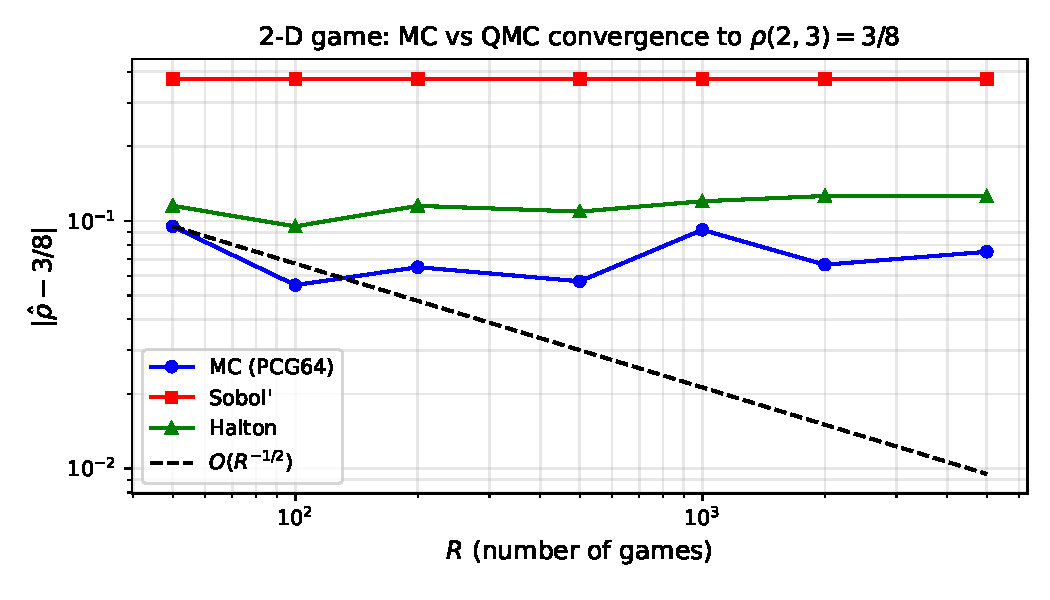
\includegraphics[width=\textwidth]{fig_game_convergence}
    \end{column}
  \end{columns}

  \framebreak

  \begin{center}
    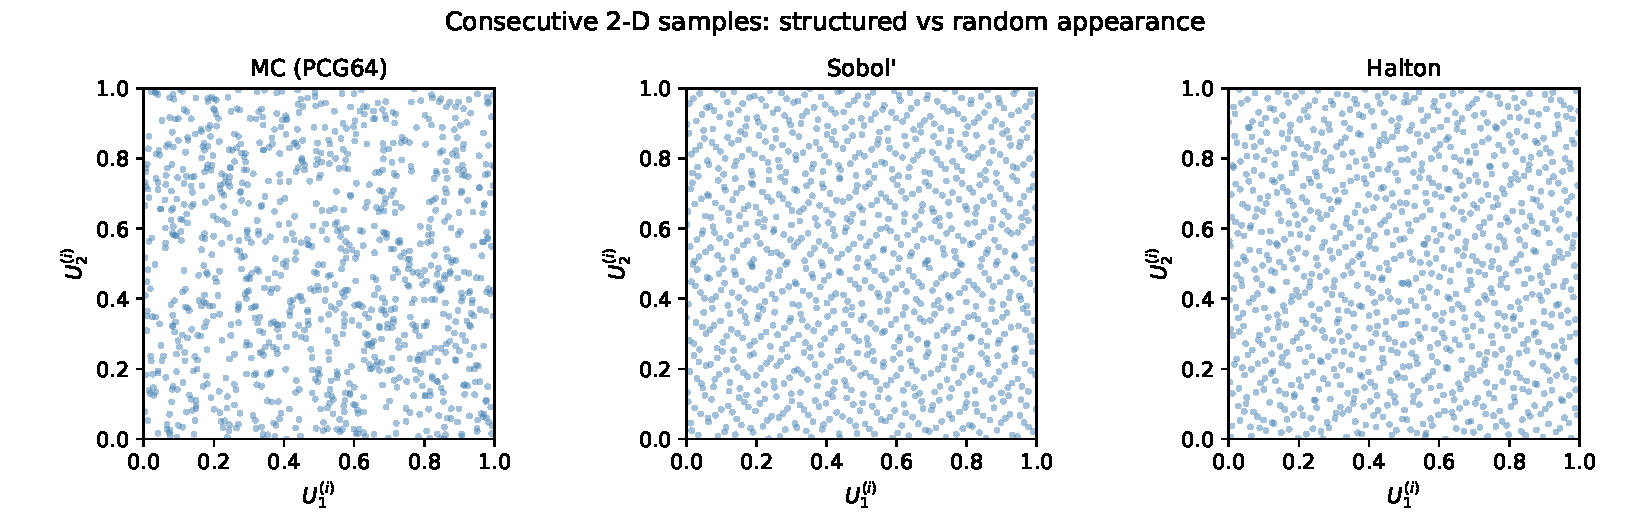
\includegraphics[width=0.85\textwidth]{fig_qmc_structure}
  \end{center}
  \textit{Scatter of consecutive sample pairs $(U_1^{(i)}, U_2^{(i)})$ for
  $n=1024$.  MC (left): unstructured. Sobol' (centre) and Halton (right):
  clear linear patterns --- a consequence of deterministic construction.
  This structure can cause artifacts when the integrand is aligned with it.}

  \begin{alertblock}{Practical rule of thumb}
    Use \textbf{QMC} for smooth, low-dimensional ($d\lesssim 5$) integrands.
    For high $d$, non-smooth $f$, or Markov-chain algorithms, prefer \textbf{MC}.
  \end{alertblock}

\end{frame}

\begin{frame}[fragile]{1.6 Python: 2-D Game -- MC vs QMC}

\begin{lstlisting}[style=python]
import numpy as np
from scipy.stats.qmc import Sobol

N1, N2 = 4, 4

def play_game(U_stream):
    i1, i2 = 2, 3
    for U1, U2 in U_stream:
        p = q = 0.25
        thr1, thr2 = 2*p, 4*p      # p1+q1, p1+q1+p2+q2
        if U1 < thr1:
            i1 += 1 if U2 < 0.5 else -1
        elif U1 < thr2:
            i2 += 1 if U2 < 0.5 else -1
        if i1 <= 0 or i2 <= 0:    return 0  # LOSE
        if i1 >= N1 and i2 >= N2:  return 1  # WIN
    return 0

def mc_estimate(R, seed=0):
    rng  = np.random.default_rng(seed)
    wins = sum(play_game(rng.random((500, 2))) for _ in range(R))
    return wins / R

print(f"MC  (R=2000): {mc_estimate(2000):.4f}")
print(f"True value : 0.3750")
\end{lstlisting}

\end{frame}

%% ==================================================================
\begin{frame}[allowframebreaks]{1.7 Bibliographical Notes}

  \textbf{Origins of Monte Carlo:}
  \begin{itemize}
    \item Developed at Los Alamos in the 1940s by von~Neumann, Ulam,
      and Metropolis. Named by Metropolis and Ulam (1949).
  \end{itemize}

  \textbf{Pseudorandom number generation:}
  \begin{itemize}
    \item Knuth [75], Vol.~2, Ch.~3: classical comprehensive reference.
    \item L'Ecuyer [82]; Niederreiter [101].
  \end{itemize}

  \textbf{Random walks and arcsine law:}
  \begin{itemize}
    \item Feller [52], Chapters~III and~XIV: arcsine law, ballot problem.
    \item Durrett [43]: modern probability, random walk results.
    \item Law of the Iterated Logarithm: [100].
  \end{itemize}

  \textbf{Quasi-Monte Carlo:}
  \begin{itemize}
    \item Niederreiter [101]: foundational QMC monograph.
    \item Halton [60]; Sobol' [119]; Faure [50].
    \item Tezuka [124]: scrambling and randomisation.
    \item Glasserman [55]: QMC for financial engineering.
    \item Python: \texttt{scipy.stats.qmc} (SciPy $\ge$ 1.7).
  \end{itemize}

  \textbf{Travelling Salesman Problem:}
  \begin{itemize}
    \item Applegate et al.\ [4]: \textit{The Traveling Salesman Problem}.
    \item Simulated annealing: Kirkpatrick, Gelatt \& Vecchi [74] (1983).
  \end{itemize}

\end{frame}

%% ==================================================================
\begin{frame}[allowframebreaks]{Chapter 1 Summary}

  \begin{block}{Core concepts}
    \begin{enumerate}
      \item \textbf{MC estimator}: $\hat{I}_R = \frac{1}{R}\sum f(U_i)$,
        RMSE $=\mathcal{O}(R^{-1/2})$, \emph{dimension-free}.
      \item \textbf{SSRW} $S_n = \sum_{j=1}^n X_j$:
        \begin{itemize}
          \item \emph{LIL}: fluctuations scale as $\pm\sqrt{2n\log\log n}$.
          \item \emph{Arcsine law}: $L^+_{2n}/(2n)$ has U-shaped arcsine
            distribution, not $\approx 1/2$.
        \end{itemize}
      \item \textbf{TSP}: NP-hard; MC heuristics (SA, CE) find near-optimal tours.
      \item \textbf{QMC}: Sobol', Halton, golden-ratio sequences achieve
        $\mathcal{O}((\log R)^d/R)$ error for smooth $f$.
      \item \textbf{MC vs QMC}: QMC wins for smooth, low-$d$ integrands;
        MC is robust for high-$d$ or non-smooth problems.
    \end{enumerate}
  \end{block}

  \framebreak

  \textbf{Key Python tools:}
  \begin{itemize}
    \item \texttt{numpy.random.default\_rng(seed)} --- reproducible PRNG
    \item \texttt{rng.random(n)}, \texttt{rng.integers(0,2,n)} --- sampling
    \item \texttt{scipy.stats.qmc.Sobol}, \texttt{.Halton}, \texttt{.LatinHypercube}
  \end{itemize}

  \bigskip
  \textbf{Coming up:}
  \begin{itemize}
    \item \textbf{Ch.~2:} How are pseudorandom numbers constructed
      and how do we test their quality statistically?
    \item \textbf{Ch.~3:} How to sample from arbitrary distributions
      (not just Uniform)?
    \item \textbf{Ch.~4:} Rigorous confidence intervals and output analysis.
  \end{itemize}

\end{frame}

\end{document}
